\subsection{General guidelines}

There is no sensitivity method that is universally suitable for all problems equally and that performs better under all conditions. 
However, in light of the methods we explore in this work, we can give general guidelines on which methods to use in specific circumstances. In this section we provide a practical overview of which methods are the most suitable for different situations. 
A simplified overview of this decision-making process is depicted in Figure \ref{fig:roadmap}. 

\begin{figure}[tb]
    \centering
    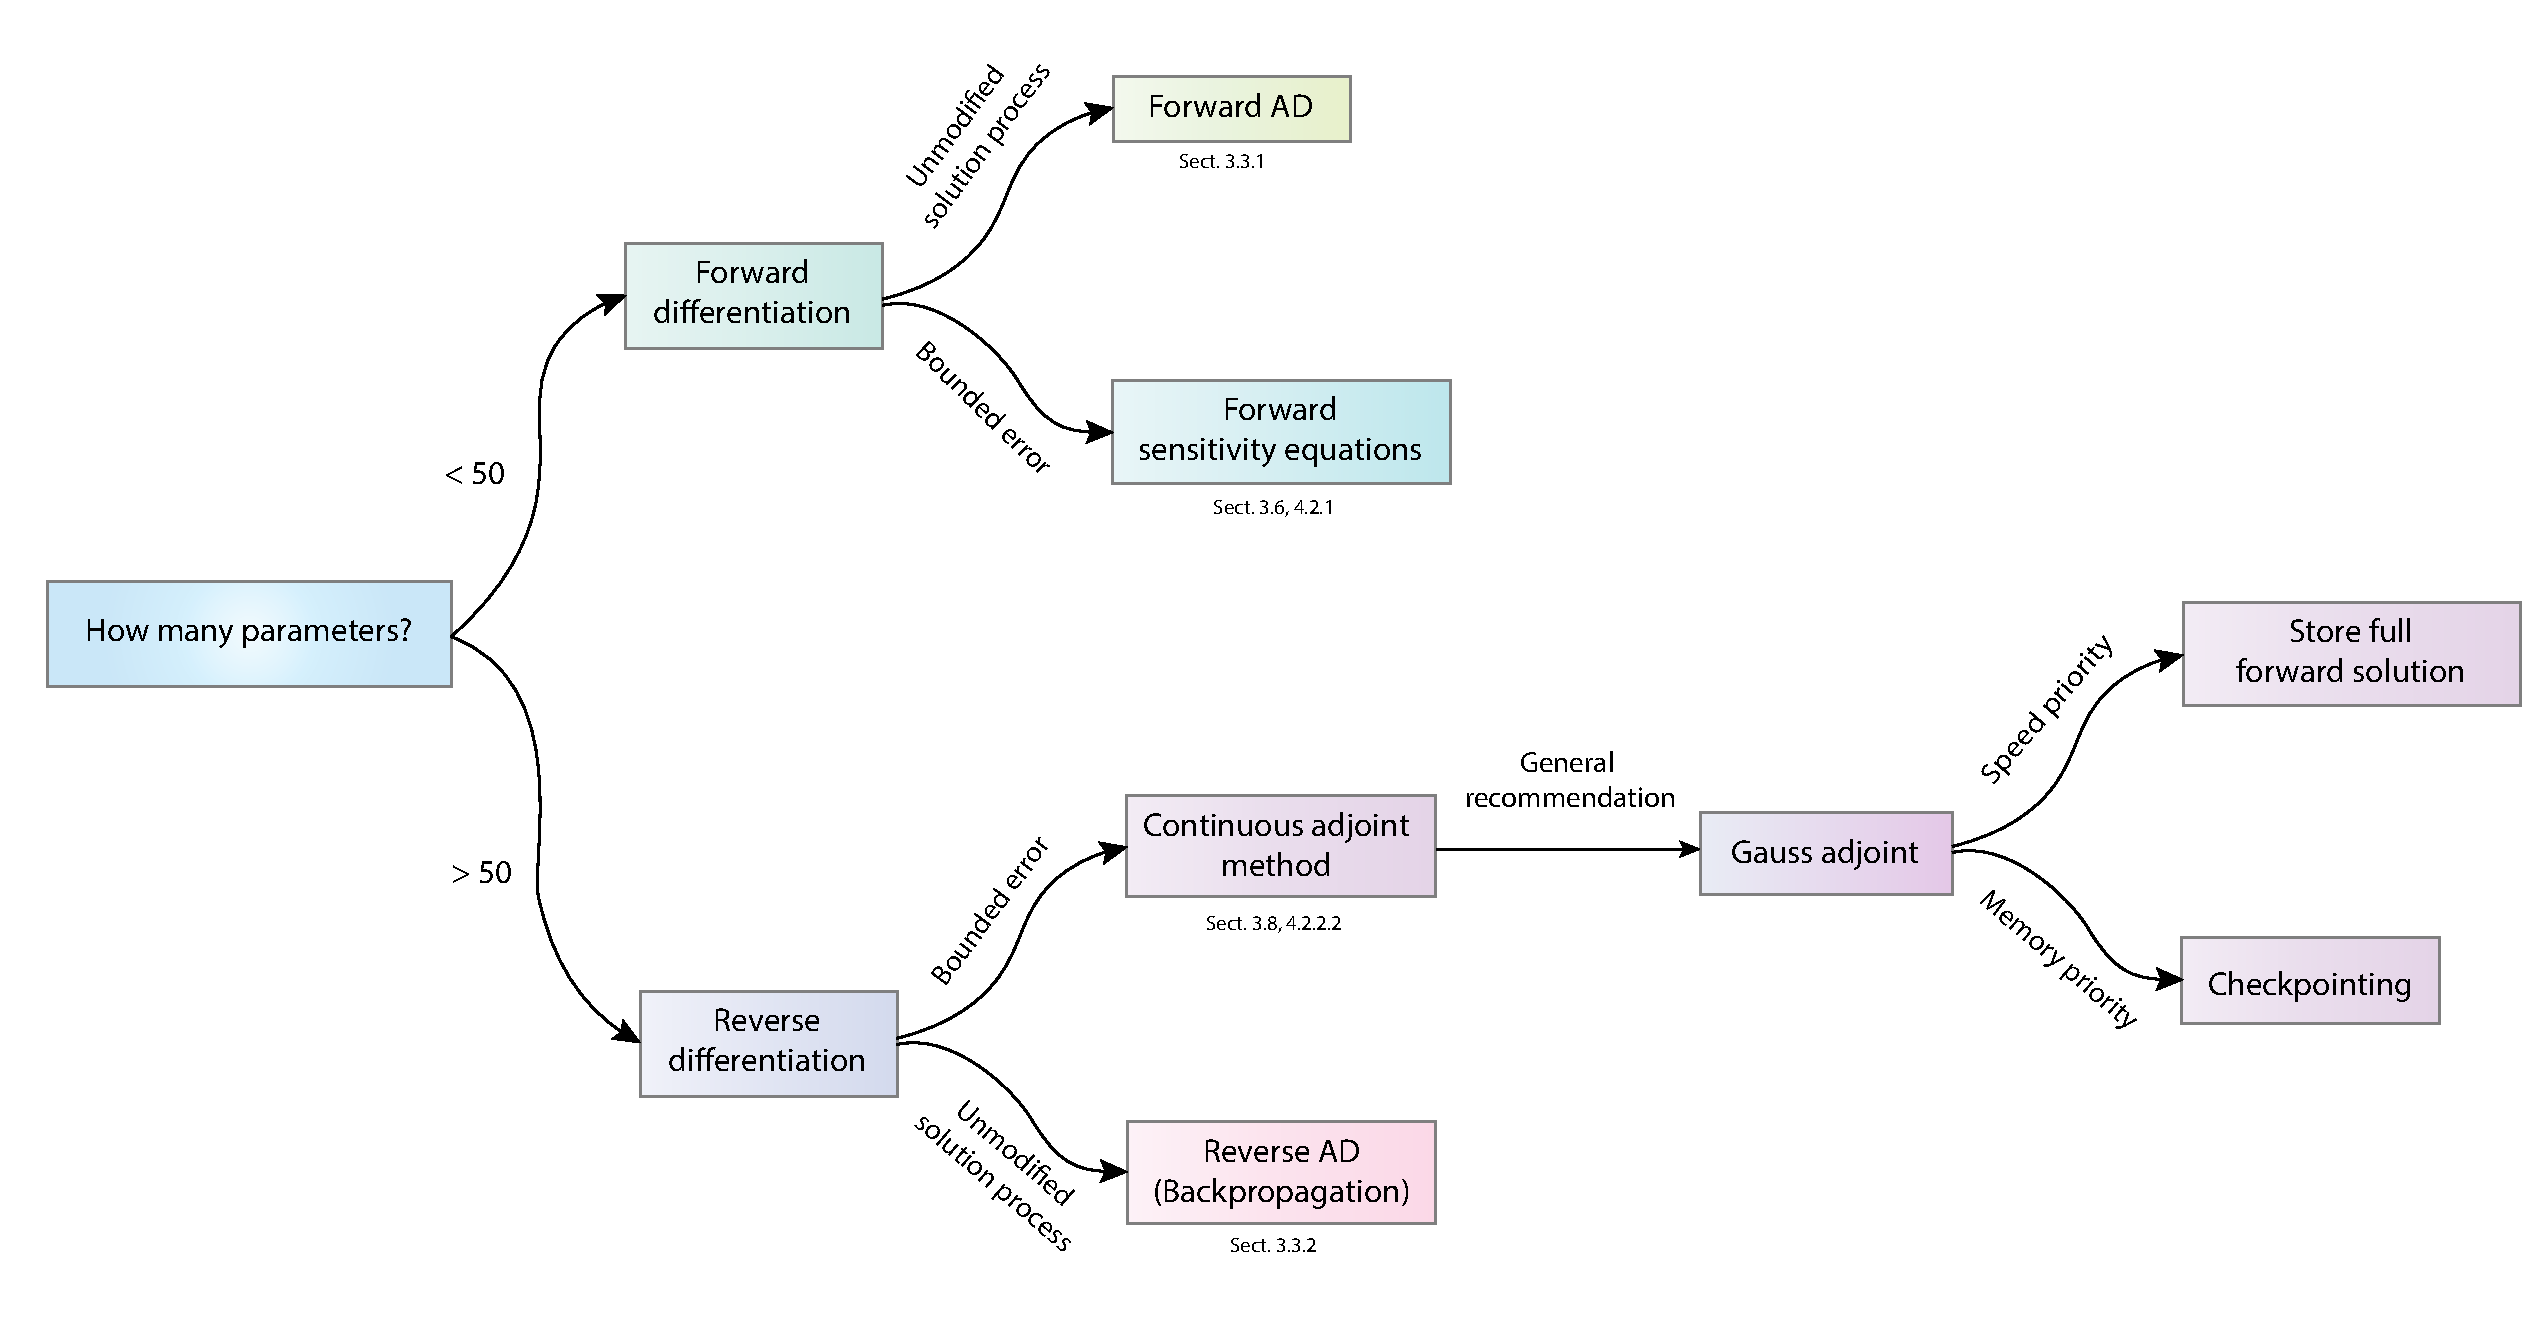
\includegraphics[width=1\textwidth]{tex/figures/roadmap.pdf}
    \caption{Decision-making tree summarizing the choice of sensitivity methods for different problems depending the type of differential equation, number of parameters, and memory-time trade-off.}
    \label{fig:roadmap}
\end{figure}

\subsubsection*{\textit{Working with small systems}}

For sufficiently small systems of less than $50$ parameters and ODEs, it has been shown that forward AD and sensitivity equations are the most efficient method, outperforming sensitivity and adjoint methods. 
The original benchmark of these methods is included in \cite{ma2021comparison}, though the \texttt{SciMLBenchmarks} system continually updates the benchmarks and has revised the cutoff point as reverse-mode AD engines improved. 
See \url{https://docs.sciml.ai/SciMLBenchmarksOutput/stable/} for continued updates.
Furthermore, as we have shown in Section \ref{section:direct-methods}, automatic differentiation outperforms other forms of direct differentiation (finite differences, complex-step differentiation). 
Modern scientific software commonly support automatic differentiation, making forward AD our preferred choice for small problems. 
We will make further comments in the choice between discrete and continuous methods later in this section.

\subsubsection*{\textit{Working with large systems}}

For larger systems with more than 50 parameters and ODEs, reverse techniques are required. 
As explained in section \ref{section:solver-methods}, the continuous adjoint method, particularly the Gauss adjoint, and for very specific cases, the interpolating adjoint and quadrature adjoint, are the most suitable methods to tackle large stiff systems. 
The choice between these three types of adjoints will be problem-specific and will depend on the trade-off between numerical stability, performance and memory usage. 
Adjoint methods supporting checkpointing present more flexibility in this sense, and can allow modulating the method depending on the performance vs memory constraints of each problem. 

Unlike for small systems of ODEs and a reduced number of parameters, differentiating large ODE systems (e.g. stiff discretized PDEs) with respect to a large number of parameters (e.g. in a neural network), is a much more complex problem. 
Current state-of-the-art tools can easily work for a wide array of small systems \cite{rackauckas2020universal}, whereas methods for large systems are still under heavy development and are likely to see many changes and improvements in the future.

Finally, it is worth mentioning that for complex stiff problems, following different strategies to avoid local minima will be absolutely necessary in order to achieve convergence (.e.g. using multiple shooting \cite{Kiehl:2006tb, Boussange2024} or progressively increasing the time span which is fitted).

\subsubsection*{\textit{Efficiency vs stability}}

When using discrete methods, it is important to be aware that the differentiation machinery is applied after the numerical solver for the differential equation has been specified, meaning that the derivatives are computed with respect to the time discretization instead of the solution \cite{Eberhard_Bischof_1996}.
As we explored in Section \ref{section:software-Forward-AD}, this can mean the method is non-convergent in the case where the iterative solver has adaptive stepsize controllers that depend on the parameter to differentiate.
Although some solutions have been proposed to solve this in the case of discrete methods \cite{Eberhard_Bischof_1996} (and have been implemented in Julia), this is a problem that continuous methods do not have since they apply the differentiation step before the numerical algorithm has been specified. 
Using many of the aforementioned \emph{tricks}, such as continuous checkpointing and Gaussian quadrature approximations, continuous sensitivity analysis tends to be more memory and computationally efficient. 
However, the errors of discrete adjoint method's derivative error may better represent the actual code being evaluated, and thus in some instances has been found to lead to more stable optimizations. 

In a nutshell, continuous adjoint methods tend to be more efficient while discrete adjoint methods tend to be more stable \cite{rackauckas2020universal}, though the opposite can apply and as such the choice ultimately depends on the nuances of each problem.



\subsubsection*{\textit{Choosing a direct method}}

When computing the gradient of a generic function other than a numerical solver, we further recommend the use of automatic differentiation (reverse or forward depending the number of parameters) as the direct method of choice, outperforming finite differences, complex step differentiation, and symbolic differentiation. 
This recommendation applies also for the inner VJPs and JVPs calculations performed inside the numerical solver (Section \ref{section:computing-vjp-inside-solver}).
As we had seen in Section \ref{section:direct-methods}, finite differences and complex step differentiation do not really provide an advantage over AD in terms of precision and require the tuning of the stepsize $\varepsilon$. 
On the other hand, if symbolic differentiation can be more efficient in nested cases (see ...) or when the spartity patter of the Jacobian is known, in general this advantage is not drastic in most real cases and can generate difficulties when used inside the numerical solver. 

However, it is important to remark that this recommendation is constraint to the availability and interoperability of different AD and sensitivity software. 
For example, when computing higher-order derivatives multiple layers of direct methods became more difficult to implement and may result in complicated computer programs.
In this cases, complex step differentiation may offer a simple alternative with similar performance than AD for small stepsizes. 

\subsubsection*{\textit{Taking into account model architecture}}

While it is important to take into account the mathematical aspects of the problem in order to choose the right type of sensitivity method, in practice, code structure and characteristics have a very strong impact in the choice of which packages to use to compute the sensitivities. 
In the context of the Julia and Python, different packages using different AD techniques will be able to deal with certain situations, while others will fail. 
Some of the most commonly encountered current limitations are the following ones:
\begin{itemize}
    \item The use of branching (i.e. \texttt{if}/\texttt{else} statements) and control flow (i.e. \texttt{for} and \texttt{while} loops) presents issues for tape-based AD methods. 
    This is currently not supported by \texttt{ReverseDiff.jl} and partially supported by \texttt{JAX} in Python. 
    Non-tape-based AD methods tend to support this, like \texttt{Enzyme.jl} and \texttt{Zygote.jl}.
    \item Mutation of arrays (i.e. in-place operations) is sometimes problematic, since it does not allow to preserve the chain rule during reverse differentation for some packages like \texttt{Zygote.jl} or \texttt{JAX}, while it is currently supported by \texttt{ReverseDiff.jl} and \texttt{Enzyme.jl}.
    \item Compatibility with GPUs (Graphical Processing Units) is still greatly under development for sensitivity methods. 
    Some AD packages like \texttt{JAX}, \texttt{Enzyme.jl} and \texttt{Zygote.jl} support it, while other packages like \texttt{ReversDiff.jl} do not. 
\end{itemize}

It is important to bear in mind that direct methods are easier to implement in programming languages where AD already exists and sometimes does not required any special package, like for the Julia programming language.
Nonetheless, users must be aware of the aforementioned convergence issues of AD naively applied to solvers. 
Thus we recommend the use of robust and tested software when available (e.g. the Julia SciML ecosystem or Diffrax in Python) as the solvers must apply corrections to AD implementations in order to guarantee numerically correct derivatives.

% Furthermore, it is important to be aware than when using AD or any other technique we are differentiating the algorithm used to lead to the numerical solution, no the numerical solution itself, which can lead to wrong results \cite{Eberhard_Bischof_1996}.
% When comparing between discrete and continuous methods, more than talking about computational efficiency we are focusing on the mathematical consistency of the method, that is, \textit{is the method estimating the right gradient?}. 
% As we will discuss in the following sections, forward methods are very efficient for problems with a small number of parameters we want to differentiate with respect to, while backwards methods are more efficient for a large number of parameters but they come with a larger memory cost which needs to be overcome using different performance tricks. 
% Neither forward nor reverse mode is more efficient in all cases \cite{Griewank_1989}, as we will discuss in Section \ref{sec:vjp-jvp}.
% When the function to differentiate has a larger input space than output ($q \ll p$), AD in reverse mode is more efficient as it propagates the chain rule by computing VJPs, the reason why reverse-mode AD is more used in modern machine learning.
%  leading to performance overhead that makes forward AD more efficient when $p \lesssim q$
% The former are easier to implement since they are agnostic with respect to the mathematical and numerical properties of the system of ODEs; however, they tend to be either inaccurate, memory-expensive, or at times unfeasible for large models. 
% which makes forward models prone to the curse of dimensionality with respect to the number of parameters considered
% For complex and large systems, direct methods for computing the gradient on top of the numerical solver can be memory expensive due to the large number of function evaluations required by the solver and the later store of the intermediate states. 


% See recommendations at \cite{Shen_diff_modelling}.

\subsection{Generalization to PDEs and DAEs}

% Generalizations to DAE \cite{Cao_Li_Petzold_2002}

\subsection{Chaotic systems}

% Integreate this paragraph in this section
% It is important to remark that adjoint methods can fail in chaotic systems \cite{Wang2012-chaos-adjoint}.
% Some works have shown that continuous adjoints can lead to unstable sensitivities \cite{Jensen_Nakshatrala_Tortorelli_2014}.
% In the more general case, discrete and continuous adjoint methods can give different computational results \cite{Sirkes_Tziperman_1997}.

% Intro: why we take this average quantities in chaotic system? Need to motivate this in a sentense.
All the sensitivity methods discussed in the previous sections encounter challenges and become less useful when applied to chaotic systems \cite{Wang2012-chaos-adjoint}.
To illustrate this, let us consider long-time-averaged quantities 
\begin{equation}\label{eq:long_time_averaged_quantities}
    \langle L(\theta) \rangle_T = \frac{1}{T} \int_0^T L(u(t), \theta) \, dt, 
\end{equation}
of chaotic systems, where $L(u(t), \theta)$ is the instantaneous objective and $u(t)$ denotes the state of the dynamical system at time $t$.
For ergodic dynamical systems, $\lim_{T\to\infty} \langle L(\theta) \rangle_T$ depends solely on the governing dynamical system and is independent of the specific choice of trajectory $u(t)$. 
In particular, $\lim_{T\to\infty} \langle L(\theta) \rangle_T$ does not depend on the initial condition. 
Under the assumption of uniform hyperbolic systems, it is possible to derive closed-form expressions and differentiability conditions for $ \langle L(\theta) \rangle_T$ \cite{ruelle1997differentiation,ruelle2009review}.
However, computing derivatives using numerical methods of statistical quantities of the form \eqref{eq:long_time_averaged_quantities} with respect to the vector parameter $\theta$ in chaotic dynamical systems remains challenging due to the \textit{butterfly effect}, i.e. small changes in the initial state or parameter can result in large differences in a later state \cite{Lorenz.1963}.
As a consequence, the solutions of the forward and adjoint sensitivity equations blow up (exponentially fast) instead of converging to the actual derivative.
To address these issues, various modifications and methods have been proposed, including approaches based on ensemble averages~\cite{lea2000sensitivity, eyink2004ruelle}, the Fokker-Planck equation~\cite{thuburn2005climate, blonigan2014probability}, the fluctuation-dissipation theorem~\cite{leith1975climate, abramov2007blended, abramov2008new}, shadowing lemma~\cite{wang2013forward, wang2014least, wang2014convergence, ni2017sensitivity, blonigan2017adjoint, blonigan2018multiple, ni2019adjoint, ni2019sensitivity}, and modifications of Ruelle's formula~\cite{chandramoorthy2022efficient, ni2020fast}.

In Julia, this is implemented in the sensitivity method \texttt{AdjointLSS} and \texttt{NILSS}. 
Standard derivative approximations are inappropriate for such systems and will not give convergent estimates.
This includes AD of a solver.